\documentclass[cs4size,a4paper,fancyhdr,fntef]{ctexbook}
\usepackage{amsmath,amsthm,amsfonts,amssymb,bm}
\usepackage{hyperref}
\usepackage[sort&compress,numbers]{natbib}
\usepackage{graphicx}
\usepackage{graphicx}
\usepackage{geometry}
\usepackage{enumitem}
\usepackage{times}
\usepackage{fancyvrb}
\usepackage{titletoc}

\makeatletter

\geometry{top=3.5cm,bottom=3.5cm,left=3.2cm,right=3.2cm}
\geometry{headheight=2.6cm,headsep=3mm,footskip=13mm}

\parskip 0.5ex plus 0.25ex minus 0.25ex

\def\cleardoublepage{\clearpage\if@twoside \ifodd\c@page\else
 \thispagestyle{empty}%
 \hbox{}\newpage\if@twocolumn\hbox{}\newpage\fi\fi\fi}


\hypersetup{CJKbookmarks,%
    bookmarksnumbered,%
        colorlinks,%
        linkcolor=black,%
        citecolor=black,%
        plainpages=false,%
        pdfstartview=FitH}


\renewcommand{\floatpagefraction}{0.80}
\newcommand\NJUTspace{\protect\CTEX@spaceChar\protect\CTEX@spaceChar}
\def\CTEX@contentsname{\zihao{3}\songti\bfseries 目\NJUTspace 录}
\def\CTEX@listfigurename{插\NJUTspace 图}
\def\CTEX@listtablename{表\NJUTspace 格}
%footnote
\fancypagestyle{plain}{%
    \fancyhf{}
    \fancyhead[C]{\if@mainmatter \small \leftmark\fi}
    \fancyfoot[C]{\small ~\thepage~}
    \renewcommand{\headrulewidth}{\if@mainmatter 0.7pt\else 0pt \fi}
}
\pagestyle{plain}

%underline
\def\NJUT@underline[#1]#2{%
    \CTEXunderline{\hbox to #1{\hfill#2\hfill}}}
\def\NJUTunderline{\@ifnextchar[\NJUT@underline\CTEXunderline}

%value
\def\NJUT@value@title{论文题目}
\def\NJUT@value@author{}
\def\NJUT@value@advisor{}
\def\NJUT@value@major{}
\def\NJUT@value@department{}
\def\NJUT@value@grade{}
\def\NJUT@value@englishtitle{}
\def\NJUT@value@englishauthor{}
\def\NJUT@value@englishadvisor{}
\def\NJUT@value@englishmajor{}
\def\NJUT@value@englishdepartment{}
\def\NJUT@value@englishgrade{}

%abstract
\def\NJUT@abs@label@bar{南京大学本科生毕业论文(设计)中文摘要}
\def\NJUT@abs@label@englishbar{南京大学本科生毕业论文(设计)英文摘要}
\def\NJUT@abs@label@title{毕业论文题目:}
\def\NJUT@abs@label@major{专业}
\def\NJUT@abs@label@department{院系}
\def\NJUT@abs@label@author{级本科生姓名:}
\def\NJUT@abs@label@advisor{指导教师 (姓名、职称):}
\def\NJUT@abs@label@abstract{摘要:}
\def\NJUT@abs@label@keywords{关键词}
\def\NJUT@abs@label@englishabstract{ABSTRACT:}
\def\NJUT@abs@label@englishkeywords{KEYWORDS:~}

\newenvironment{abstract}{
    \pdfbookmark[0]{\NJUT@abs@label@abstract}{abstract}
    \begin{center}
        {\bf\kaishu\zihao{-2} \uuline{\NJUT@abs@label@bar}}
    \end{center}

    {\kaishu\zihao{4}%
        \noindent \NJUT@abs@label@title \NJUTunderline[315pt]{\NJUT@value@title}

        \noindent \NJUTunderline[400pt]{}

        \noindent \NJUTunderline[85pt]{\NJUT@value@department}\NJUT@abs@label@department%
        \NJUTunderline[71pt]{\NJUT@value@major}\NJUT@abs@label@major%
        \NJUTunderline[43pt]{\NJUT@value@grade}\NJUT@abs@label@author%
        \NJUTunderline[60pt]{\NJUT@value@author}

        \noindent \NJUT@abs@label@advisor \NJUTunderline[252pt]{\NJUT@value@advisor}

        \NJUT@abs@label@abstract

    }
}{}
\newcommand\keywords[1]{\vspace{2ex}\noindent{\kaishu \NJUT@abs@label@keywords} #1}

\newenvironment{englishabstract}{%
    \clearpage
    \begin{center}
        {\bf\kaishu\zihao{-2} \uuline{\NJUT@abs@label@englishbar}}
    \end{center}
    {\zihao{4}%
    \begin{description}[font=\normalfont,leftmargin=4em]
        \item[THESIS:]\NJUT@value@englishtitle
        \item[DEPARTMENT:]\NJUT@value@englishdepartment
        \item[SPECIALIZATION:]\NJUT@value@englishmajor
        \item[UNDERGRADUATE:]\NJUT@value@englishgrade
        \item[MENTOR:]\NJUT@value@englishadvisor
        \item[ABSTRACT:]\hfil
    \end{description}
    }
}{}
\newcommand\englishkeywords[1]{%
    \vspace{2ex}\noindent{\NJUT@abs@label@englishkeywords} #1}

%%
%contents
%%

\newcommand\NJUTtableofcontents{%
\@mainmattertrue
\addcontentsline{toc}{chapter}{目\NJUTspace 录}
\@mainmatterfalse
\tableofcontents
}
\addtocontents{toc}{\let\string\CTEX@spaceChar\relax}

\titlecontents{chapter}[2em]
              {\addvspace{0.6pc}\heiti\bfseries\zihao{4}}
              {\thecontentslabel\enspace}
              {}
              {\titlerule*[0.5em]{$\cdot$}\contentspage}
              [\addvspace{0.25pc}]

\titlecontents{section}[4em]
              {\addvspace{0.1pc}\songti\zihao{-4}}
              {\thecontentslabel\enspace}
              {}
              {\titlerule*[0.5em]{$\cdot$}\contentspage}
              [\addvspace{0.25pc}]

\newcommand\Nchapter[1]{%
    \if@mainmatter%
        \@mainmatterfalse%
        \chapter{#1}%
        \@mainmatterture%
    \else
        \chapter{#1}%
    \fi}
%bib
\renewcommand\bibfont{\zihao{-4}}
\def\CTEX@references{\zihao{1}参考}

%%section
\setcounter{secnumdepth}{4}
\def\CTEX@chapter@nameformat{\bfseries\heiti\zihao{4}}
\def\CTEX@chapter@titleformat{\bfseries\heiti\zihao{4}}
\def\CTEX@chapter@beforeskip{15\p@}
\def\CTEX@chapter@afterskip{12\p@}
\def\CTEX@section@format{\bfseries\heiti\zihao{4}\centering}
\def\CTEX@section@beforeskip{-3ex \@plus -1ex \@minus -.2ex}
\def\CTEX@section@afterskip{1.0ex \@plus .2ex}
\def\CTEX@subsection@format{\bfseries\heiti\zihao{-4}}
\def\CTEX@subsection@indent{2\ccwd}
\def\CTEX@subsection@beforeskip{-2.5ex \@plus -1ex \@minus -.2ex}
\def\CTEX@subsection@afterskip{1.0ex \@plus .2ex}
\def\CTEX@subsubsection@format{\bfseries\heiti\zihao{-4}}
\def\CTEX@subsubsection@indent{2\ccwd}
\def\CTEX@subsubsection@beforeskip{-2ex \@plus -1ex \@minus -.2ex}
\def\CTEX@subsubsection@afterskip{1.0ex \@plus .2ex}



\newtheoremstyle{break}% name
{}% Space above, empty = `usual value'
{}% Space below
{\itshape}% Body font
{}% Indent amount (empty = no indent, \parindent = para indent)
{\bfseries}% Thm head font
{.}% Punctuation after thm head
{\newline}% Space after thm head: \newline = linebreak
{}% Thm head spec


%%
%% the theorems definitions
%%
\theoremstyle{plain}
\newtheorem{algo}{算法~}[chapter]
\newtheorem{thm}{定理~}[chapter]
\newtheorem{lem}[thm]{引理~}
\newtheorem{prop}[thm]{命题~}
\newtheorem{cor}[thm]{推论~}
\theoremstyle{definition}
\newtheorem{defn}{定义~}[chapter]
\newtheorem{conj}{猜想~}[chapter]
\newtheorem{exmp}{例~}[chapter]
\newtheorem{rem}{注~}
\newtheorem{case}{情形~}
\theoremstyle{break}
\newtheorem{bthm}[thm]{定理~}
\newtheorem{blem}[thm]{引理~}
\newtheorem{bprop}[thm]{命题~}
\newtheorem{bcor}[thm]{推论~}
\renewcommand{\proofname}{{\bf 证明}} 

\makeatother
\usepackage{algorithm}
\usepackage{algorithmic}
\usepackage{perpage}
\usepackage{float}


\MakePerPage{footnote}

\def \x {\bm{ x}}

\def \A {\bm{ A}}
\def \B {\bm{ B}}
\def \C {\bm{C}}
\def \W {\bm{ W}}
\def \V {\bm{ V}}
\def \bv {\bm{ v}}
\def \bh {\bm{ h}}
\def \bb {\bm{b}}
\def \bP {\bm{P}}
\def \bQ {\bm{Q}}
\def \bL {\bm{L}}
\def \bF {\bm{F}}
\def \bg {\bm{g}}
\def \bI {\bm{I}}
\def \R {\bm{R}}

\newcommand\upp[1]{^{(#1)}}
\newcommand\norm[1]{\lVert#1\rVert}
\newcommand\inner[1]{\langle #1\ \rangle}
\DeclareMathOperator*{\argmin}{\arg\!\min}

\def \bxi {\boldsymbol{\xi}}
\def \btau {\boldsymbol{\tau}}
\def \balpha {\boldsymbol{\alpha}}
\def \1 {{\bf 1}}
\def \0 {{\bm 0}}


\begin{document}
\bibliographystyle{NJUthesis}
\CTEXsetup[format+={\flushleft}]{section}
\frontmatter
\begin{abstract}
\kaishu\zihao{-4}
C-TOMO(Computed Tomography,即计算机断层扫描)是一种医学影像技术。
它通过X射线所产生数据来计算被投射物体的断层影像。
由于断层影像给诊断、观测所带来的便利,C-TOMO技术被广泛应用于医疗领域。
各领域对于C-TOMO技术所产生的图像质量也有了越来越高的要求。小角度的C-TOMO技术有助于减少
C-TOMO成像的成本,但在图像质量上不如全角度的C-TOMO,会出现边界模糊等问题,此外,由于
X射线的扫描方向限制,在某些方向上的断层图像质量也较为不好。在C-TOMO计算时,我们还可以
采用一些其他手段获得关于被测的物体的一些先验知识,如果能够将这些先验知识以某种形式应用到成像
的过程中,并使之约束C-TOMO成像的过程,则可以使成像结果获得提升。本论文是针对特定的三维物体,
以超声成像(US,UltraSound)的数据作为先验知识进行的小角度C-TOMO成像。对于成像算法,我采用改进
的SART迭代算法,通过提取超声成像的梯度信息,并将之作为SART迭代优化过程中的约束条件,正则化为优化目标
,从而明显改进了成像的质量,也把US图像的优势融合到了C-TOMO成像之中。

\keywords{计算机断层扫描,小角度,先验知识,优化,SART算法,超声成像}
\end{abstract}

\begin{englishabstract}

\end{englishabstract}
\NJUTtableofcontents
\mainmatter
\chapter{绪论}
\section{背景介绍}
众所周知,在X-射线被发现后,人们就将之应用于医学上的人体透视检测。然后,直接使用X射线,会直接减少一个维度
信息,对于很多细微部分的检测会出现很大问题。于是有不少研究者开始探寻从X射线的投影中生成横向断层切片图像的
方法。Radon在1917的一篇文献中提出了断层摄影(tomography)的数学工作(\cite{radon1986},为后来的断层影像生成
提供了基础。在断层摄影中,可以根据获得的投影图像生成探测物体的内部结构。断层摄影相比于传统的投影图像存在着
三个优点,第一,它可以提供足够的深度定位;第二,它
可以极大提高探测物体的可视性;第三,通过调整动态范围,它可以提高局部组织的对比度,
从而可以更好进行观测。很快,因为它在人体内部检测的巨大优势,
它迅速被医疗领域所使用\cite{dobbins2003digital}。

随后,在这个方法的基础上人们
改进并不断提出了新的方法,如带滤波的反向投影算法(Filtered Backprojection, FBP)\cite{kak1979computerized}。

\chapter{基于SART的优化算法}
\section{算法概述}
在SART算法的基础上,改进了一种优化算法,该算法可以把超声成像的信息融合到重建的过程中,从而在重建中可以
引导重建图像的生成,使得重建以一种合理的方式融合X射线tomography与超声成像的优势,由此来弥补小角度成像所造成
的信息缺失。下面是本文所提出的优化算法的基本框架。
\begin{algo}\label{mysart}
基于SART的优化算法
\begin{algorithmic}[1]
\STATE
Initialize $\x^{(0)} \leftarrow \bm{0}$,$t\leftarrow \bm{0}$
\REPEAT
\STATE
$\bL(\x^{(t)}) \leftarrow  \V^{-1}\A^T\W(\bb-\A\x^{(t)})$ \\
$\bP(\x^{(t)}) \leftarrow \B^{T}(\bh-\B\x^{(t)})$ \\    %水平
$\bQ(\x^{(t)}) \leftarrow \C^{T}(\bv-\C\x^{(t)})$         %垂直
\STATE
$\x^{(t+1)}\leftarrow \omega\bL(\x^{(t)}) + \lambda\bP(\x^{(t)}) + \xi\bQ(\x^{(t)})    $
\UNTIL{convergence}
\end{algorithmic}
\end{algo}

在算法\ref{mysart}中,$\x$代表的是所重建的数据,为一维向量,是将立体的物体模型以确定方向的坐标延伸而成。
$\bL(x^{(k)})$,分别是tomo约束的迭代增量,而$\bP(x^{(k)})$和$ \bQ(x^{(k)})$是超声数据的信息
的迭代增量\footnote{在算法中可以增加多个先验知识,在本文中我们使用了两个信息,分别为超声数据的不同方向所提取的,
具体见章节\ref{sec:mysart},后同。}。矩阵$\A$是在Tomography中X射线的投影矩阵,$\V$是对角矩阵,它的对角元素
是$V_{j,j}=A_{+,j}$,$\W$也是对角矩阵,其元素为$V_{j,j}=A_{i,+}$,$\B,\C$是提取超声信息所用的矩阵,
$\bh,\bv$则是超声信息中所提取出来信息,也是一维向量。
$\omega,\lambda_h,\lambda_v$
分别是三者的迭代步进参数。关于该算法的细节在接下来的章节中进一步描述。
\section{使用梯度信息的基于SART的优化算法}\label{sec:mysart}
在前所述的研究工作中,我们发现:
\begin{enumerate}
    \item 由于X射线tomography是小角度重建的原因,本质上信息是缺失的。在我们的模型中所直接看到的情况就是肿块
    在垂直方向上的大小变化不清晰,并没有清楚的变化边缘,而是呈现逐渐模糊掉的形式。这点是超声数据可以弥补的,
    它在肿块边界的变化上有明显的优势。
    \item 超声重建的探测方向与x射线tomography的探测方向并不相同。x射线tomography的探测方向是在被测物体上方往下
    放射,而放射管在一个小角度里转动。相比之下超声重建的探测方向是被测物体的边上以垂直于tomography的方向发射的,
    由此可以知道两者在物体不同部分的信息也并不相同。特别是在经过了两者数据的配准之后,在沿超声探测方向上实际上已经
    有了插值数据,而这些数据实际上如果完全应用于重建是不合理的。
    \item 物体内不同材料对X射线和超声的吸收特性是不一样的,甚至可能会呈现相反的趋势。
    \item 超声重建后的数据存在着不小的噪声。
\end{enumerate}
在上述讨论中,我们可以发现,直接应用超声数据到重建中是不合理的,因为超声数据有许多冗余的信息会误导到tomo重建。同时,
我们可以发现,我们所需要的是超声重建数据的边缘信息。超声数据对肿块清晰的边缘可以弥补tomography重建中肿块边缘信息的缺失,
同时即使材料对X射线和超声的吸收特性不同,不同材料之间的边缘信息也是一致的。因此,如果能有效利用边缘信息,我们便可以把
超声信息的优势加入到数据重建中。

为了利用边缘信息,将使用图像的梯度作为要提取的信息。在图~\ref{fig:model}中,我们看到超声是沿着$y$轴进行探测,由此超声重建数据
在$x,z$方向上的梯度具有较多的有用信息。特别是在$z$方向上的梯度,包含有肿块在$z$方向上的变化信息,这可以对tomogarphy重建的肿块在
这个方向上边缘变化不明显的问题做一个比较好的补偿。

在算法~\ref{mysart}中,有$\bh,\bv$实际上就是超声提取的梯度信息,这个是直接对超声重建的数据取梯度并经过一定的处理完成的一维向量
\footnote{直接得到的梯度图像包含有大量的噪声,还不能直接使用,需要经过处理,见章节\ref{sec:gradprocess}}。
而$\B,\C $则是对图像取梯度的矩阵算子。

\section{算法展开}\label{sec:algodetail}
将算法~\ref{mysart}根据前述章节内容展开,我们将得到每一次迭代的过程如下:
\begin{align}
 L_k(x_i) &= \cfrac{1}{A_{+,k}}\sum^N_{i=1}\cfrac{A_{i,k}}{A_{i,+}}\bigl(b_i-\bar{b_i}(x\upp{t})\bigr) \label{eq:L} \\
P_k(x_i^{(t)}) &= \begin{cases}
                            -(2x_k\upp{t} - x_{k+mn}\upp{t} - x_{k-mn}\upp{t} - h_k + h_{k-mn}) & mn \le k \le N-mn \\
                            -(x_k\upp{t} - x_{k+mn}\upp{t} - h_k) &  k\le mn \\
                            -(x_{k-mn}\upp{t} - x_{k}\upp{t} - h_{k-mn}) &  N-mn \le k \le N
                        \end{cases}  \label{eq:P} \\
Q_k(x_i^{(t)}) &= \begin{cases}
                            -(2x_k\upp{t} - x_{k+n}\upp{t} - x_{k-n}\upp{t} - v_k + v_{k-mn}) & k \notin [ imn-n+1, imn+n]
                            \\ &i = 0,1,2\hdots\\
                            -(x_k\upp{t} - x_{k+n}\upp{t} - v_k) & k \in \left[imn+1,imn+n\right] \\ &i = 0,1,2\hdots\\
                            -(x_{k-n}\upp{t} - x_{k}\upp{t} - v_{k-n}) &  k \in [imn-n+1,imn] \\ &i= 1,2,3 \hdots
                        \end{cases} \label{eq:Q} \\
x_k^{(t+1)}&= x_k\upp{t} + \omega L_k(x^{(t)}) + \lambda P_k(x^{(t)}) + \xi Q_k(x^{(t)}) \label{eq:all}
\end{align}
其中$m,n$分别是被测立方物体底面的两边长度,$m$为$x$方向上的边长,$n$为$y$方向上的边长。$N$为物体所有的像素点数。

上述就是基于SART的优化算法采用两个方向的梯度信息的结果。方程\eqref{eq:L}, \eqref{eq:P}, \eqref{eq:Q}分别给出了三项的展开结果,其中方程
\eqref{eq:P}, \eqref{eq:Q}是已经将梯度运算矩阵$\B,\C$代入的结果。而方程
\eqref{eq:all}将三项的迭代项通过步进参数调整后加到$\x$上进行迭代。可以看到,该算法的展开结果与SART算法相比,
是在SART的基础上增加了两项超声梯度信息项,这两项超声梯度信息项将超声的梯度信息融合到了重建中。在后面的部分中我们可以看到,这种
算法可以使得被重建的物体将在满足tomograph投影约束。
\begin{equation*}
\A\x = \bb
\end{equation*}
与两个梯度约束
\begin{align*}
\B\x &= \bh \\
\C\x &= \bv
\end{align*}
中取得全局最优化的结果。
\section{优化目标的建立}\label{sec:optobj}
在章节\ref{sec:algodetail}中,提到了被重建的物体需要满足tomograph投影约束与两个梯度约束,在这三个约束中间取到最优化。事实上,基于约束
的优化也正是SART算法的本质所在。我们知道,在tomography的投影探测中,X射线穿过物体,并被沿途的被测物体物质进行一定量的吸收,最后发射
到传感器上,传感器检测到射线的吸收量。由此,这个吸收量其实就是被物体该射线所穿过的每个像素沿着探测射线进行累积(积分)的量。由于我们
需要采用数值方法计算,物体的像素被我们离散,所以这个吸收量实际上就是射线途径的物体像素的累积和。对于每一条射线,我们都
可以用一个相应的矩阵来代表它的路径。它实际上就是与物体等大小的一个矩阵。我们将物体的像素写成一位列向量$\x$的形式后,该矩阵实际上就变成
了与之等长的一个行向量。将所有探测光束所代表的横向量进行排列以后,实际上就得到了我们的投影约束矩阵$\A$。而相应的得到的投影数据也
写成一个一维列向量的形式$\bb$。因此,我们得到了方程
\begin{equation}
\A\x = \bb \label{eq:tomocon}
\end{equation}
此外,在章节\ref{sec:mysart}中提到,我们要将超声数据的梯度信息融合到重建中。实际上,就是要使得重建的物体的固定方向的梯度上要与超声数据
对应方向的梯度相接近。考虑到SART算法实际上是解决这样一个优化问题:
\begin{equation}
\x = \argmin_{\x\in R^N}\W\norm{\A\x-\bb}^2 \label{eq:sartopt}
\end{equation}
方程\eqref{eq:sartopt}的优化其实是一个带权的最小平方误差优化,权$\W$ 是因为SART的形式需要加上。这个优化,实际上就是在寻找一个值$\x$,它能使得$\A\x$与得到的投影数据 $\bb$的相差最小。在本文中,将它的范数定为损失函数。
注意范数函数都为凸函数,因此这是一个凸优化。
将梯度的约束加上,我们就得到
\begin{equation}
\x = \argmin_{\x\in R^N}\W\norm{\A\x-\bb}^2 +\norm{\B\x-\bh}^2+\norm{\C\x-\bv}^2 \notag
\end{equation}
实际上,这样并不是最合理的,因为这样可能会使得最后的数据偏向tomo的约束方向或者偏向梯度约束方向。注意我们是要使得重建的数据在一定程度上
被引向梯度约束,因此,可以在上面的优化目标中增加参数$c,d$用来控制各个约束对数据的影响程度,这些参数可以在实验中确定一个最佳值,因此
,方程变为
\begin{equation}
\x = \argmin_{\x\in R^N}\W\norm{\A\x-\bb}^2 +c\norm{\B\x-\bh}^2+d\norm{\C\x-\bv}^2 \qquad c>0,d>0 \label{eq:mysartopt}
\end{equation}
注意在方程\eqref{eq:mysartopt}中,它由于是多个范数的非负权重和,因此它还是一个凸函数\cite{boyd2004convex},这仍然是一个凸优化。而为了解决
这个优化问题,我们将使用梯度下降算法\cite{nesterov2003}。
\section{梯度下降算法}\label{sec:graddescent}
我们知道,负梯度$-f'(x)$是函数下降最快的方向。因此,如果要求目标最小值的话,
可以将被优化目标往它的负梯度方向每次步进一些,就能到达一个局部最小值,
梯度下降算法框架如下:
\begin{algo}
对于一个可微的优化目标 $f(x)$
\begin{algorithmic}[1]
\STATE
选择一个$x_{0}\in R^n$
\STATE
迭代\\
$x_{k+1}=x_{k}-h_kf'(x_{k}),\qquad k=0,1,\hdots$
\end{algorithmic}
\end{algo}
其中$h_k$被称为step size,步进大小。它的值可以挑选合适的,比如
\begin{align*}
h_k &= h>0,\quad h\text{为常数}\\
h_k &= \cfrac{h}{\sqrt{k+1}}
\end{align*}
在\cite{nesterov2003}中给出了梯度下降算法的性能分析。定义
$C^{k,p}_L(Q)$是一族$k$阶可微函数,其第$p$阶导数在$Q$上满足Lipschitz
连续,也就是
\begin{equation*}
\norm{f\upp{p}(x)-f\upp{p}(y)}\le L\norm{x-y}\qquad \text{对于所有的} x,y\in Q
\end{equation*}
考虑这个优化问题
\begin{equation}\label{eq:gdopt}
\min_{x\in R^n}f(x)
\end{equation}
其中$f(x)\in C^{1,1}_L(R^n)$,我们假设$f(x)$在$R^n$上有下界,且步进参数
为常数。由$y=x-hf'(x)$,从上述假设里首先我们可以得出
\begin{equation}
\begin{split} \label{eq:une}
f(y) &\le f(x) + \inner{f'(x),y-x}+\frac{L}{2}\norm{y-x}^2  \\
     &= f(x)-h\norm{f'(x)}^2+\frac{h^2}{2}L\norm{f'(x)}^2 \\
     &= f(x)-h(1-\frac{h}{2}L)\norm{f'(x)}^2
\end{split}
\end{equation}
因此,为了估计最佳的下降大小,我们需要解这个一维问题:
\begin{equation*}
\Delta (h)=-h(1-\frac{h}{2}L)\rightarrow\min_h
\end{equation*}
取这个函数的导数,我们可以得到$\Delta '(h)=hL-1=0$,因此,解
是$h^\star=\frac{1}{L}$,同时这也是$\Delta(h)$的最小值。

因此,前式变为
\begin{equation*}
f(y)\le f(x)-\cfrac{1}{2L}\norm{f'(x)}^2
\end{equation*}
当考虑之前的迭代策略$x_{k+1}=x_k-h_kf'(x_k)$,$h_k=h$代入,有:
\begin{equation*}
f(x_k)-f(x_{k+1})\ge h(1-\cfrac{1}{2}Lh)\norm{f'(x_k)}^2
\end{equation*}
现在考虑一般情况下的情况。由上面的集中类型我们可以得到
\begin{equation}
f(x_k)-f(x_{k+1})\ge \cfrac{\omega}{L}\norm{f'(x_k)}^2
\end{equation}
其中$\omega$是一个正常数。

将上面的式子以$k=0,\hdots,N$累加起来,可以得到
\begin{equation}
\cfrac{\omega}{L}\sum^N_{k=0}\norm{f'(x_k)}^2\le f(x_0)-f(x_N)
\le f(x_0)-f^\star
\end{equation}
其中$f^\star$是对问题\eqref{eq:gdopt}的最优化值。因此,
由上式我们可以得出
\begin{equation*}
\norm{f'(x_k)}\rightarrow 0 \qquad k\rightarrow \infty
\end{equation*}
也就是说,被优化函数的梯度$f'(x)$可以在一定次数的迭代之后趋向于$0$。定义收敛序列
\begin{equation*}
g^\star_N=\min_{0\le k\le N}g_k
\end{equation*}
其中$g_k=\norm{f'(x_k)}^2$。于是,可以得到下述不等式:
\begin{equation}
g^\star_N \le \cfrac{1}{\sqrt{N+1}}[\cfrac{1}{\omega}L(f(x_0)-f^\star)]^{1/2}
\end{equation}
上市右边项提示了$g^\star_N$与$N$的关系。

在\cite{nesterov2003}中还对梯度下降算法的收敛性进行了分析。有定理
\begin{thm}\label{thm:graddecent}
令函数$f(x)$满足如下的假设:
\begin{enumerate}
\item{$f\in C^{2,2}_M(R^n)$}
\item{存在函数$f$的局部最小值,且在这个点上它的Hessian是正定的}
\item{存在一些边界$0<l\le L<\infty$,对于在点$x^\star$的Hessian来说,有
\begin{equation*}
lI_n\le f''(x^\star)\le LI_n
\end{equation*}}
\end{enumerate}
且令$x_0$足够接近局部最小值:
\begin{equation*}
r_0=\norm{x_0-x^\star}<\bar{r}=\cfrac{2l}{M}
\end{equation*}
于是使用合适的步进值的梯度下降方法可以以如下的速率收敛:
\begin{equation*}
\norm{x_k-x^\star}\le \cfrac{\bar{r}r_0}{\bar{r}-r_0}(1-\cfrac{l}{L+l})^k
\end{equation*}
\end{thm}
也就是说,梯度下降算法是线性收敛的。在章节\ref{eq:optobj}中提到,我们的目标函数为多个范数非负权相加的形式。由于范数
函数本身是凸的,所以这个非负权和的形式也是凸的。我们知道,凸函数有一个特点,是有唯一全局最小点。因此,采用梯度下降
算法所收敛到的局部最小点就是全局最小点。同时,我们也在定理\ref{thm:graddecent}中看到梯度下降算法具有优良的收敛性,
因此使用梯度下降算法解这个优化问题是合理的。另外,在后文中我们会看到SART算法本身的形式也是能利用梯度下降算法来解释,
这也更进一步增加了使用梯度下降算法的合理性。
\section{基于SART的优化算法推导}
接下来将采用梯度下降算法来推导出算法\ref{mysart}。重新将优化目标\ref{eq:mysartopt}写在这里
\begin{equation}
\min_{\x\in R^N}\W\norm{\A\x-\bb}^2 +c\norm{\B\x-\bh}^2+d\norm{\C\x-\bv}^2 \qquad c>0,d>0
\end{equation}
我们令
\begin{equation*}
\bF(\x) = \W\norm{\A\x-\bb}^2 +c\norm{\B\x-\bh}^2+d\norm{\C\x-\bv}^2
\end{equation*}
它是一个连续可微的函数,所以我们求它的梯度
\begin{equation*}
\nabla \bF(\x) = 2(\A^T\W(\A\x-\bb)+c\B^T(\B\x-\bh)+d\C^T(\C\x-\bv))
\end{equation*}
使用梯度下降,我们有
\begin{equation}\label{eq:gradout}
\begin{split}
\x\upp{t+1}&=\x\upp{t}-\cfrac{\omega}{2}\V^{-1}\nabla F(\x\upp{t})\\
&=\x\upp{t} + \omega\V^{-1}\A^T\W(\bb-\A\x\upp{k})
           + c\omega\V^{-1}\B^T(\bh-\B\x)
           + d\omega\V^{-1}\C^T(\bv-\C\x)
\end{split}
\end{equation}\label{eq:gradfinal}
令$\lambda = c\omega\V^{-1},\xi = d\omega\V^{-1}$
于是方程\eqref{eq:gradout}变为
\begin{equation}\label{eq:gradout2}
\x\upp{t+1}= \x\upp{t} + \omega\V^{-1}\A^T\W(\bb-\A\x\upp{k})
           + \lambda \B^T(\bh-\B\x\upp{k})
           + \xi \C^T(\bv-\C\x\upp{k})
\end{equation}
可以发现,方程\eqref{eq:gradfinal}其实就是算法\ref{mysart}
的迭代过程。在其中,为了能得到SART基础项的正确形式,设置步进常数为$\tfrac{\omega}{2}\V^{-1}$,
这样可以使得正常的SART可以不被破坏\footnote{SART的设置本身具有良好的收敛性,这点我们在后文中会提到},而
在上面的最后一步中,我们将$\omega\V^{-1}$和梯度相自带的
常数$c,d$(可以是矩阵)一起合并成一个简单的常数项$\lambda ,\xi$,这个步骤实际上就是一定程度
上把梯度项的迭代和tomogaphy的投影项的迭代过程分离开来。如果常数项选择不当的话,轻的后果是可能使得其中一些项的作用超过其它项,而
严重的话则从定理
\ref{thm:graddecent}中,我们可以知道,会使得
迭代过程不再收敛。可以发现,我们的优化目标中含有矩阵$\A$,它是一个复杂的大矩阵(tomography投影矩阵),
此外,还带有权矩阵$\W$,这与梯度项所带的梯度计算矩阵$\B,\C$的数量级往往并不一样,所以优化目标将变的较为复杂,
直接采用解析的方法计算合理的步进常数项是难以实现的,因此,将在实验中确定合理的参数项。

下面将推导出该算法的展开具体展开形式。首先要给出计算梯度的计算。先分析$\x$的排列。我们知道,它是将三维的物体数据伸展成一维的。物体的模型
示意见图\ref{fig:model1}。
\begin{figure}[ht]
\center
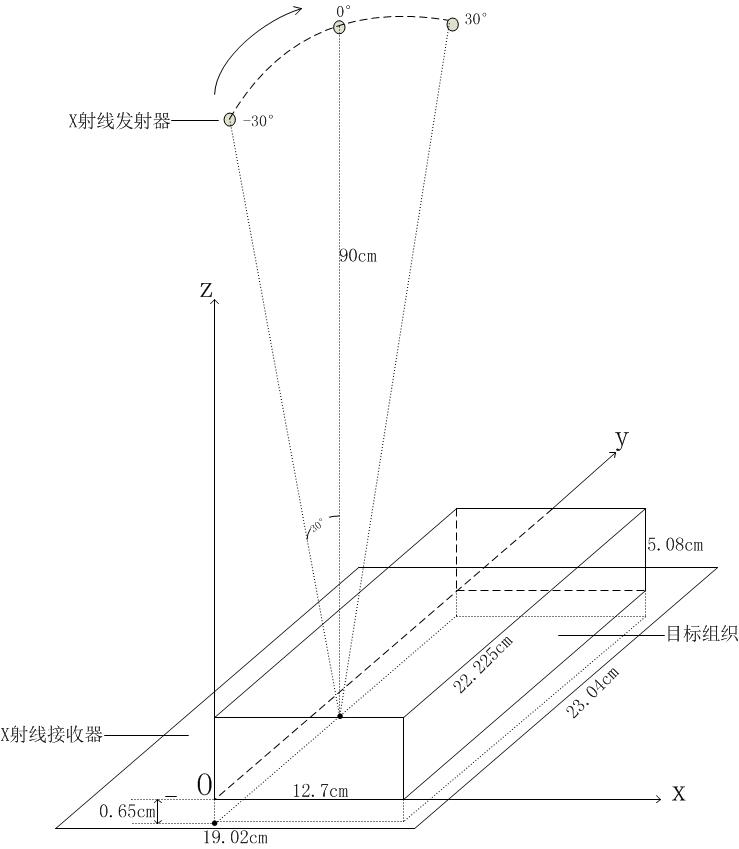
\includegraphics[width=0.8\textwidth]{figure/model1.jpg}
\caption{探测物体模型}\label{fig:modle1}
\end{figure}
在图中,探测物体在$x$方向的边长为$m$,在$y$方向的边长为$n$。注意图中沿$y$轴的三根箭头,三维物体的像素索引顺序是依照此箭头进行的。也就是说,索引顺序的第一级顺序是$y$轴正方向顺序,第二级顺序是$x$
轴正方向顺序,第三级顺序是$z$轴正方向顺序。对于一个在物体中的坐标标号为$I_{xyz}$的的像素点而言,它在$\x$中的坐标索引$x_i$计算方式如下:
\begin{equation}\label{eq:indexconvert}
x_i = I_{xyz}\qquad \text{当} i = mnz+nx+y
\end{equation}
从取梯度的角度考虑,我们不选择超声探测平行的方向梯度信息,这是因为探测本身的积分特性,会使得在这个方向上相对被模糊,也就是
梯度信息不如与超声探测方向相垂直的方向。由于超声影像的探测方向是沿着$y$轴正方向照射,我们选择在$x$,$z$两个方向的梯度信息。

首先处理沿着$z$轴的梯度方向。要计算沿着该方向的梯度。实际上就是对于所计算出来的梯度$grad$,这样的:
\begin{equation}\label{eq:grad_z1}
grad_{xyz} = I_{xyz}-I_{xy(z+1)}
\end{equation}
方程\eqref{eq:grad_z1}没有涉及到最后一个平面的问题。一般来说,梯度的边缘并不是十分重要,因此,为了方便未来的计算,将边缘处补$0$。
由式\eqref{eq:indexconvert}可以得到:
\begin{equation}\label{eq:grad_z2}
g_i = \begin{cases}
        x_{i} - x_{i+mn} & i \le N-mn \\
        0   & i \in [N-mn+1,N]
        \end{cases}
\end{equation}
对于式\eqref{eq:grad_z2},可以写成矩阵形式:
\begin{equation*}
\bg = \C \x
\end{equation*}
其中矩阵$\C$如下:
\begin{equation*}
\C = \begin{pmatrix}
1 & 0 & 0 & 0 & \cdots &-1 & 0 &0 &0 &\cdots \\
0 & 1 & 0 & 0 &\cdots &0 & -1 &0 &0 &\cdots \\
\hdotsfor[3]{3}& 1& \cdots &\hdotsfor[3]{3}&-1&\cdots \\
0 & 0 & 0 & \hdotsfor[3]{5}&0&0 \\
\hdotsfor[3]{10}\\
\hdotsfor[3]{10}\\
0 & 0 & \ddots & 0 & \cdots & 0 & 0 & \ddots & 0& \cdots
\end{pmatrix}
\end{equation*}
或者可以写成
\begin{equation*}
\C = \begin{pmatrix}
\bI &  -\bI & \0 & \0 & \0 \cdots \\
\0 & \bI &  -\bI & \0 & \0 \cdots \\
\0 & \0  & \ddots & \ddots & \0 & \cdots \\
\hdotsfor[3]{7} \\
\0 & \0 & \0 &\cdots & \0 & \0 &\0 \cdots
\end{pmatrix}
\end{equation*}
其中,$\bI$是一个大小为$mn * mn$的单位矩阵,而$bm 0$ 则是大小为$mn * mn$的零矩阵。
于是我们可以得到关于$\C$ 矩阵的归纳式:
\begin{equation}\label{eq:C}
C_{ij} = \begin{cases}
1 & i = j,\quad i\le N-mn \\
-1 & i = j- mn,\quad i\le N- mn \\
0 & \text{其它}
\end{cases}
\end{equation}

接下来是$\B$矩阵的推导。对于$\B$,其求梯度方向是沿着$x$轴方向。同样的,为了未来计算方便,在边缘处补$0$。
这个边缘也就是物体沿着$x$轴的最外侧。类似于$\C$,可以得到:
\begin{equation*}
\B = \begin{pmatrix}
1 & 0 & 0 & 0 & \cdots &-1 & 0 &0 &0 &\cdots \\
0 & 1 & 0 & 0 &\cdots &0 & -1 &0 &0 &\cdots \\
0 & 0 & \ddots & 0 & \cdots & 0 & 0 & \ddots & 0& \cdots \\
\hdotsfor[3]{3}& 1& \cdots &\hdotsfor[3]{3}&-1&\cdots \\
0 & 0 & 0 & \hdotsfor[3]{5}&0&0 \\
\hdotsfor[3]{10}\\
\hdotsfor[3]{10}
\end{pmatrix}
\end{equation*}
为了方便描述,也可以写成矩阵形式:
\begin{equation*}
\B = \begin{pmatrix}
\tilde{\bI} &  -\tilde{\bI} & \0 & \0 & \0 \cdots \\
\0 & \tilde{\bI} &  -\tilde{\bI} & \0 & \0 \cdots \\
\0 & \0  & \ddots & \ddots & \0 & \cdots \\
\hdotsfor[3]{7} \\
\0 & \0 & \0 &\cdots & \0 & \0 &\0 \cdots
\end{pmatrix}
\end{equation*}
其中,$\tilde{\bI}$是一个大小为$n * n$的矩阵,描述如下:
\begin{equation*}
\tilde{\bI} = \begin{pmatrix}
1 & 0 & 0 & \cdots &\cdots & \cdots\\
0 & 1 & 0 & \cdots &\cdots & \cdots\\
 & &\ddots & \\
& & & \cdots& 1 & 0 \\
0 & \cdots & \cdots & \cdots & \cdots & 0
\end{pmatrix}
\end{equation*}
而$\bm 0$ 则是大小为$n * n$的零矩阵。于是$\B$可以写成归纳形式如下:
\begin{equation}\label{eq:B}
B_{ij} = \begin{cases}
1 & i=j, \quad i \notin [kmn-n+1,kmn] \\
-1 & i = j-n \quad i \notin [kmn-n+1,kmn] \\
0 & \text{其它}
\end{cases}
\end{equation}

现在,矩阵$\B$和$\C$ 都已经得到了,我们需要对式子\eqref{eq:gradout2}作进一步展开,并得到可以计算的最终结果。

考虑式子
\begin{equation*}
\B^T(\bh-\B\x)
\end{equation*}
先将内部展开,根据$\B$ 的定义,可以得到:
\begin{equation*}
\begin{split}
(\bh-\B\x)_i &= -(\sum_{j=1}^{N}B_{ij}x_j - h_i)\\
             & = \begin{cases}
             -(x_i -x_{i+n} -h_i)  & i \notin [kmn-n+1,kmn]\\
             0  & \text{其它} \\
             \end{cases} \\
             & = T_i
\end{split}
\end{equation*}
再展开的式子的外层,有
\begin{equation*}
(\B^T(\bh-\B\x))_j = \sum_{j=1}^{N}\B_{ij}T_i \\
\end{equation*}
考虑到$\B$ 定义,即式子\eqref{eq:B},上式可以进一步展开为
\begin{equation*}
\sum_{j=1}^{N}\B_{ij}T_i =  \begin{cases}
T_j -T_{j-n} & j\notin [kmn-n+1,kmn+n]\\
T_j  & j \in [kmn+1,kmn+n] \\
-T_{j-n} & j \in [kmn-n+1,kmn]
\end{cases}
\end{equation*}
将上述式子进一步展开,就得到
\begin{equation} \label{eq:Bout}
(\B^T(\bh-\B\x))_j = \begin{cases}
-(2x_j -x_{j+n} -x_{j-n} -h_j + h_{j-n}) & j\notin [kmn-n+1,kmn+n]\\
-(x_j-x_{j+n}-h_j) & j \in [kmn+1,kmn+n] \\
(x_{j-n}-x_j-h_{j-n} & j \in [kmn-n+1,kmn]
\end{cases}
\end{equation}

接下来考虑式子
\begin{equation*}
\C^T(\bh-\C\x)
\end{equation*}
先将内部展开,根据$\C $的定义,可以得到:
\begin{equation*}
\begin{split}
(\bv-\C\x)_i &= -(\sum_{j=1}^{N}C_{ij}x_j - v_i)\\
             & = \begin{cases}
             -(x_i -x_{i+mn} -v_i)  & i \notin [N-mn+1,kmn]\\
             0  & \text{其它} \\
             \end{cases} \\
             & = Y_i
\end{split}
\end{equation*}
再展开的式子的外层,有
\begin{equation*}
(\C^T(\bv-\C\x))_j = \sum_{j=1}^{N}\C_{ij}Y_i \\
\end{equation*}
考虑到$\C$ 定义,即式子\eqref{eq:C},上式可以进一步展开为
\begin{equation*}
\sum_{j=1}^{N}\C_{ij}Y_i =  \begin{cases}
Y_j -Y_{j-n} & j\in [mn,N-mn]\\
Y_j  & j \in [1,mn] \\
-Y_{j-mn} & j \in [N-mn,N]
\end{cases}
\end{equation*}
将上述式子进一步展开,就得到
\begin{equation} \label{eq:Cout}
\C^T(\bh-\C\x))_j = \begin{cases}
-(2x_j -x_{j+mn} -x_{j-mn} -v_j + v_{j-n}) & j\in [mn,N-mn]\\
-(x_j-x_{j+mn}-v_j) & j \in [1,mn] \\
(x_{j-mn}-x_j-v_{j-mn} & j \in [N-mn,N]
\end{cases}
\end{equation}

对于式子\eqref{eq:gradout2}中的第一项,我们可以直接展开得到:
\begin{equation}\label{eq:Aout}
(\omega\V^{-1}\A^T\W(\bb-\A\x))_j = \cfrac{\omega}{A_{+,j}}
\sum_{i=1}^M\cfrac{A_{i,j}}{A_{i,+}}(b_i-\bar{b}_i(x))
\end{equation}
在上式中
\begin{align*}
A_{i,+}=\sum_{j=1}^N{A_{i,j}} \\
A_{+,j}=\sum_{i=1}^M{A_{i,j}} \\
\bar{b}_i(x)=(\A\x)_i
\end{align*}
其中$N,M$分别表示矩阵$A$的横、纵长度。矩阵$A$是投影矩阵,将在具体问题中获得,
在章节\ref{sec:obtainA}中会详细介绍。

于是,将式\eqref{eq:Aout}式\eqref{eq:Bout}以及式\eqref{eq:Cout}代入到式\eqref{eq:gradout2}中,
就可以得到我们算法的完整展开形式了。
\section{基于SART算法的收敛性}
在章节\ref{sec:graddescent}中,已经提到了梯度下降算法的收敛性在一定的条件下(该条件一般都满足)是线性时间的。
而SART算法本身就是一种梯度下降算法,加在其前面的是相应的矩阵项$\V^{-1}$,其实是相当于在最小平方误差中的每一个维度
分别添加了一个相应的参数。而对于SART迭代项的收敛性,在论文\cite{jiang2003convergence}中对其做了详细的总结与证明。

\cite{jiang2003convergence}中中先证明了SART算法解的存在性。
令$N(A)$是矩阵$\A$的零空间,则根据正交分解理论有:
\begin{equation*}
\R^N=N(A)\bigoplus N(A)^\perp
\end{equation*}
其中$N(A)^\perp$表示$N(A)$的正交补子空间,令$R(\A^T)$表示矩阵$\A^T$的值域,
所以,可以知道$N(A)^\perp=R(\A^T)$

令
\begin{equation*}
L(x)=\sum_{i=1}^M\cfrac{1}{A_{i,+}}(b_i-\bar{b}_i(x))^2=\norm{\bb-\A\x}^2_W
\end{equation*}
其中$\norm{\bb-\A\x}^2_W = \W\norm{\bb-\A\x}^2$,它的梯度表示为:
\begin{equation*}
\nabla L(\x)=-2\A^T\W(\bb-\A\x)
\end{equation*}
而所有$L$的最小化点要满足
\begin{equation}\label{eq:normaleq}
\A^T\W\A\x=\A^T\W\bb
\end{equation}
因为$\inner{\A^T\W\A\x,\x}=\norm{\A\x}^2_W$,因此可以得到$N(A^TWA)=N(A)$。
且因为$\A^T\W\bb\in R(\A^T) = N(A)^\perp$,\ref{eq:normaleq}存在解。

令S为\eqref{eq:normaleq}的解集。
则由于$L(x)$是在$\x$上的凸函数,\eqref{eq:normaleq}
的解也是$L$的最小化点,反之亦然。所以$S$也是$L$在$\R^N$上的最小化点集。

接下\cite{jiang2003convergence}中证明了SART算法的收敛性问题。其中有:
\begin{equation*}
L(x\upp({x}))-L(x\upp{k})\le -\alpha\norm{x\upp{k+1}-x\upp{k}}^2_V
\end{equation*}
其中$\alpha = 2/\omega -1 > 0$。又有下述推论:
\begin{enumerate}
\item{$\{L(x\upp{k})\}^\infty_{k=0}$有界。}
\item{$L(x\upp{k+1})\le L(x\upp{k})$}
\item{\begin{equation*}
L(x\upp{k+1})+\alpha\sum^k_{j=0}\norm{x\upp{j+1}-x\upp{j}}^2_V\le L(x_0)
\end{equation*}}
\item{$\sum^\infty_{j=0}\norm{x\upp{j+1}-x\upp{j}}^2_V$收敛}
\item{\begin{equation*}
\norm{x\upp{k+1}-x\upp{k}}\rightarrow 0,\text{对于}k\rightarrow \infty
\end{equation*}}
\end{enumerate}

\bibliography{thesis}
\end{document}



